\documentclass[]{article}
\usepackage{lmodern}
\usepackage{amssymb,amsmath}
\usepackage{ifxetex,ifluatex}
\usepackage{fixltx2e} % provides \textsubscript
\ifnum 0\ifxetex 1\fi\ifluatex 1\fi=0 % if pdftex
  \usepackage[T1]{fontenc}
  \usepackage[utf8]{inputenc}
\else % if luatex or xelatex
  \ifxetex
    \usepackage{mathspec}
  \else
    \usepackage{fontspec}
  \fi
  \defaultfontfeatures{Ligatures=TeX,Scale=MatchLowercase}
\fi
% use upquote if available, for straight quotes in verbatim environments
\IfFileExists{upquote.sty}{\usepackage{upquote}}{}
% use microtype if available
\IfFileExists{microtype.sty}{%
\usepackage{microtype}
\UseMicrotypeSet[protrusion]{basicmath} % disable protrusion for tt fonts
}{}
\usepackage[margin=1in]{geometry}
\usepackage{hyperref}
\hypersetup{unicode=true,
            pdftitle={Managing for ecological surprises in metapopulations},
            pdfborder={0 0 0},
            breaklinks=true}
\urlstyle{same}  % don't use monospace font for urls
\usepackage{color}
\usepackage{fancyvrb}
\newcommand{\VerbBar}{|}
\newcommand{\VERB}{\Verb[commandchars=\\\{\}]}
\DefineVerbatimEnvironment{Highlighting}{Verbatim}{commandchars=\\\{\}}
% Add ',fontsize=\small' for more characters per line
\usepackage{framed}
\definecolor{shadecolor}{RGB}{248,248,248}
\newenvironment{Shaded}{\begin{snugshade}}{\end{snugshade}}
\newcommand{\KeywordTok}[1]{\textcolor[rgb]{0.13,0.29,0.53}{\textbf{#1}}}
\newcommand{\DataTypeTok}[1]{\textcolor[rgb]{0.13,0.29,0.53}{#1}}
\newcommand{\DecValTok}[1]{\textcolor[rgb]{0.00,0.00,0.81}{#1}}
\newcommand{\BaseNTok}[1]{\textcolor[rgb]{0.00,0.00,0.81}{#1}}
\newcommand{\FloatTok}[1]{\textcolor[rgb]{0.00,0.00,0.81}{#1}}
\newcommand{\ConstantTok}[1]{\textcolor[rgb]{0.00,0.00,0.00}{#1}}
\newcommand{\CharTok}[1]{\textcolor[rgb]{0.31,0.60,0.02}{#1}}
\newcommand{\SpecialCharTok}[1]{\textcolor[rgb]{0.00,0.00,0.00}{#1}}
\newcommand{\StringTok}[1]{\textcolor[rgb]{0.31,0.60,0.02}{#1}}
\newcommand{\VerbatimStringTok}[1]{\textcolor[rgb]{0.31,0.60,0.02}{#1}}
\newcommand{\SpecialStringTok}[1]{\textcolor[rgb]{0.31,0.60,0.02}{#1}}
\newcommand{\ImportTok}[1]{#1}
\newcommand{\CommentTok}[1]{\textcolor[rgb]{0.56,0.35,0.01}{\textit{#1}}}
\newcommand{\DocumentationTok}[1]{\textcolor[rgb]{0.56,0.35,0.01}{\textbf{\textit{#1}}}}
\newcommand{\AnnotationTok}[1]{\textcolor[rgb]{0.56,0.35,0.01}{\textbf{\textit{#1}}}}
\newcommand{\CommentVarTok}[1]{\textcolor[rgb]{0.56,0.35,0.01}{\textbf{\textit{#1}}}}
\newcommand{\OtherTok}[1]{\textcolor[rgb]{0.56,0.35,0.01}{#1}}
\newcommand{\FunctionTok}[1]{\textcolor[rgb]{0.00,0.00,0.00}{#1}}
\newcommand{\VariableTok}[1]{\textcolor[rgb]{0.00,0.00,0.00}{#1}}
\newcommand{\ControlFlowTok}[1]{\textcolor[rgb]{0.13,0.29,0.53}{\textbf{#1}}}
\newcommand{\OperatorTok}[1]{\textcolor[rgb]{0.81,0.36,0.00}{\textbf{#1}}}
\newcommand{\BuiltInTok}[1]{#1}
\newcommand{\ExtensionTok}[1]{#1}
\newcommand{\PreprocessorTok}[1]{\textcolor[rgb]{0.56,0.35,0.01}{\textit{#1}}}
\newcommand{\AttributeTok}[1]{\textcolor[rgb]{0.77,0.63,0.00}{#1}}
\newcommand{\RegionMarkerTok}[1]{#1}
\newcommand{\InformationTok}[1]{\textcolor[rgb]{0.56,0.35,0.01}{\textbf{\textit{#1}}}}
\newcommand{\WarningTok}[1]{\textcolor[rgb]{0.56,0.35,0.01}{\textbf{\textit{#1}}}}
\newcommand{\AlertTok}[1]{\textcolor[rgb]{0.94,0.16,0.16}{#1}}
\newcommand{\ErrorTok}[1]{\textcolor[rgb]{0.64,0.00,0.00}{\textbf{#1}}}
\newcommand{\NormalTok}[1]{#1}
\usepackage{graphicx,grffile}
\makeatletter
\def\maxwidth{\ifdim\Gin@nat@width>\linewidth\linewidth\else\Gin@nat@width\fi}
\def\maxheight{\ifdim\Gin@nat@height>\textheight\textheight\else\Gin@nat@height\fi}
\makeatother
% Scale images if necessary, so that they will not overflow the page
% margins by default, and it is still possible to overwrite the defaults
% using explicit options in \includegraphics[width, height, ...]{}
\setkeys{Gin}{width=\maxwidth,height=\maxheight,keepaspectratio}
\IfFileExists{parskip.sty}{%
\usepackage{parskip}
}{% else
\setlength{\parindent}{0pt}
\setlength{\parskip}{6pt plus 2pt minus 1pt}
}
\setlength{\emergencystretch}{3em}  % prevent overfull lines
\providecommand{\tightlist}{%
  \setlength{\itemsep}{0pt}\setlength{\parskip}{0pt}}
\setcounter{secnumdepth}{0}
% Redefines (sub)paragraphs to behave more like sections
\ifx\paragraph\undefined\else
\let\oldparagraph\paragraph
\renewcommand{\paragraph}[1]{\oldparagraph{#1}\mbox{}}
\fi
\ifx\subparagraph\undefined\else
\let\oldsubparagraph\subparagraph
\renewcommand{\subparagraph}[1]{\oldsubparagraph{#1}\mbox{}}
\fi

%%% Use protect on footnotes to avoid problems with footnotes in titles
\let\rmarkdownfootnote\footnote%
\def\footnote{\protect\rmarkdownfootnote}

%%% Change title format to be more compact
\usepackage{titling}

% Create subtitle command for use in maketitle
\newcommand{\subtitle}[1]{
  \posttitle{
    \begin{center}\large#1\end{center}
    }
}

\setlength{\droptitle}{-2em}

  \title{Managing for ecological surprises in metapopulations}
    \pretitle{\vspace{\droptitle}\centering\huge}
  \posttitle{\par}
  \subtitle{Supplemental materials}
  \author{Kyle Logan Wilson\(^1\), Colin Bailey\(^1\), William Atlas\(^1\), and
Doug Braun\(^2\)\\[2\baselineskip]\(^1\)Earth to Ocean Research Group,
Simon Fraser University\\
\(^2\)Fisheries \& Oceans Canada}
    \preauthor{\centering\large\emph}
  \postauthor{\par}
      \predate{\centering\large\emph}
  \postdate{\par}
    \date{01 May 2019}

\let\origfigure\figure
\let\endorigfigure\endfigure
\renewenvironment{figure}[1][2] {
    \expandafter\origfigure\expandafter[H]
} {
    \endorigfigure
}

\begin{document}
\maketitle

\subsection{Metapopulation model}\label{metapopulation-model}

\subsubsection{Local \& metapopulation
dynamics}\label{local-metapopulation-dynamics}

Our metapopulation is defined by a set of local populations \(N_p\) with
time-dynamics that follows birth (i.e., recruitment \emph{R}),
immigration, death, and emigration (BIDE) processes:

\(N_{it}= R_{it}\epsilon_{it}+I_{it}-D_{it}-E_{it}\)

where \(N_{it+1}\) is the number of adults in patch \emph{i} at time
\emph{t}, \(R_{it}\) is number of recruits, \(I_{it}\) is number of
recruits immigrating into patch \emph{i} from any other patch,
\(D_{it}\) is number of recruits that die due to disturbance regime,
\(E_{it}\) is the number of recruits emigrating from patch \emph{i} into
any other patch, and \(\epsilon_{it}\) is stochasticity in recruitment.

Resoure monitoring often occurs at the scale of the metapopulation,
hence we define metapopulation adults as:

\({MN}_t = \sum_{i=1}^{N_p} N_{it}\)

with metapopulation recruits:

\(MR_t = \sum_{i=1}^{N_p} R_{it}\)

Local patch recruitment at time \emph{t} depended on adult densities at
\emph{t-1} and followed a reparameterized Beverton-Holt function:

\(R_{it}=\cfrac{\alpha_iN_{it-1}}{1+\cfrac{\alpha_i-1}{\beta_i}N_{it-1}}\)

where \(\alpha_i\) is the recruitment compensation ratio and \(\beta_i\)
is local patch carrying capacity.

For example, in a two patch model that varies \(\alpha_i\) and
\(\beta_i\) parameters such that

\begin{Shaded}
\begin{Highlighting}[]
\NormalTok{alpha <-}\StringTok{ }\KeywordTok{c}\NormalTok{(}\DecValTok{2}\NormalTok{, }\DecValTok{4}\NormalTok{)}
\NormalTok{beta <-}\StringTok{ }\KeywordTok{c}\NormalTok{(}\DecValTok{100}\NormalTok{, }\DecValTok{200}\NormalTok{)}
\end{Highlighting}
\end{Shaded}

Management often monitors metapopulation resources as the aggregate of
all local populations. In this way, recruitment compensation from local
patches \(\alpha_i\) gets averaged across the metapopulation leading
mean compensation \(\bar{\alpha}\) of 3. Likewise, the total carrying
capacity of the metapopulation \(\bar{\beta}\) becomes the summation of
local patch carrying capacities \(\beta_i\), which is 300. This scale of
monitoring generates the following local patch and metapopulation
dynamics:

\begin{wrapfigure}{R}{0.7\textwidth}[H]

\hfill{}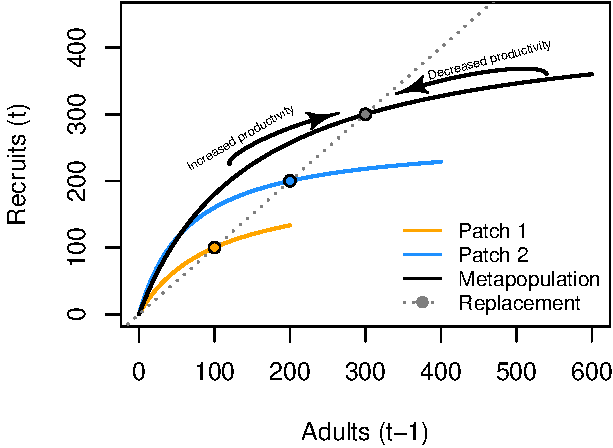
\includegraphics[width=.7\textwidth,trim = {0 1.1cm 0 0}, clip]{Managing_for_ecological_surprises_in_metapopulations_files/figure-latex/recruit curves-1} 

\caption{Metapopulation and local patch recruitment dynamics.}\label{fig:recruit curves}
\end{wrapfigure}

\subsubsection{Creating the spatial
networks}\label{creating-the-spatial-networks}

The next aspect to our metapopulation model is connecting the set of
patches to one another. We need to specify the number of patches, their
arrangements (i.e., connections), and how far apart they are from one
another. We followed some classic metapopulation and source-sink
arrangements to create four networks that generalize across a few
real-world topologies: a linear habitat network (e.g., coastline), a
dendritic or branching network (e.g., coastal rivers), a star network
(e.g., mountain \& valley), and a complex network (e.g., terrestrial
plants).

To make networks comparable, each spatial network type needs the same
leading parameters (e.g., \(N_p\) and \(\bar{d}\)) . In this case for
number of patches, we set \(N_p\) to \texttt{16} and \(\bar{d}\) to
\texttt{1} unit (distance units are arbitrary). We used the
\texttt{igraph} package and some custom code to arrange our spatial
networks as the following:

\begin{figure}
\centering
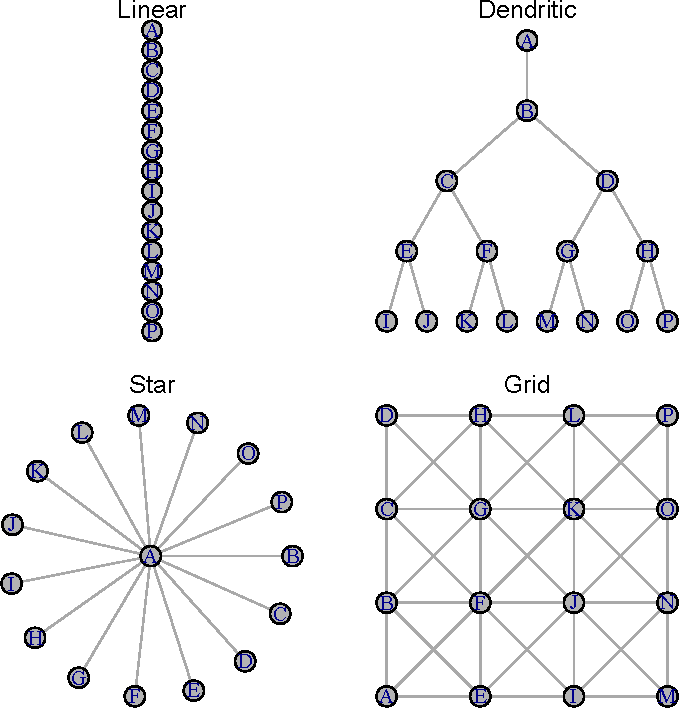
\includegraphics{Managing_for_ecological_surprises_in_metapopulations_files/figure-latex/networks-1.pdf}
\caption{Four spatial network topologies.}
\end{figure}

Note that distances between each connecting patch (the links between
nodes) in the above networks are equal.

An example dispersal matrix for the complex network:

\begin{verbatim}
##   A B E F C G D H I J K L M N O P
## A 0 1 1 1 2 2 3 3 2 2 2 3 3 3 3 3
## B 1 0 1 1 1 1 2 2 2 2 2 2 3 3 3 3
## E 1 1 0 1 2 2 3 3 1 1 2 3 2 2 2 3
## F 1 1 1 0 1 1 2 2 1 1 1 2 2 2 2 2
## C 2 1 2 1 0 1 1 1 2 2 2 2 3 3 3 3
## G 2 1 2 1 1 0 1 1 2 1 1 1 2 2 2 2
## D 3 2 3 2 1 1 0 1 3 2 2 2 3 3 3 3
## H 3 2 3 2 1 1 1 0 3 2 1 1 3 2 2 2
## I 2 2 1 1 2 2 3 3 0 1 2 3 1 1 2 3
## J 2 2 1 1 2 1 2 2 1 0 1 2 1 1 1 2
## K 2 2 2 1 2 1 2 1 2 1 0 1 2 1 1 1
## L 3 2 3 2 2 1 2 1 3 2 1 0 3 2 1 1
## M 3 3 2 2 3 2 3 3 1 1 2 3 0 1 2 3
## N 3 3 2 2 3 2 3 2 1 1 1 2 1 0 1 2
## O 3 3 2 2 3 2 3 2 2 1 1 1 2 1 0 1
## P 3 3 3 2 3 2 3 2 3 2 1 1 3 2 1 0
\end{verbatim}

\subsubsection{Dispersal}\label{dispersal}

Dispersal from patch \emph{i} into patch \emph{j} depends on constant
dispersal rate \(\omega\) (defined as the proportion of total local
recruits that will disperse) and an exponential distance-decay function
between \emph{i} and \emph{j} with distance cost to dispersal \(m\)
following:

\(E_{ij(t)}=\omega R_{it}p_{ij}\)

with probability of dispersal from patch i into patch j:

\(p_{ij}=\dfrac{e^{-md_{ij}}}{\sum\limits_{\substack{j=1 \\ j\neq i}}^{N_p} e^{-md_{ij}}}\)

where \(d_{ij}\) is the pairwise distance between patches and \(E_{ij}\)
is the total dispersing animals from patch i into patch j. The summation
term in the denominator normalizes the probability of moving to any
patch to between 0 and 1. With \(\bar{d}= 1\), \(m=0.5\),
\(\omega=0.1\), \(R_{it}=100\) in a linear network:

\begin{figure}
\centering
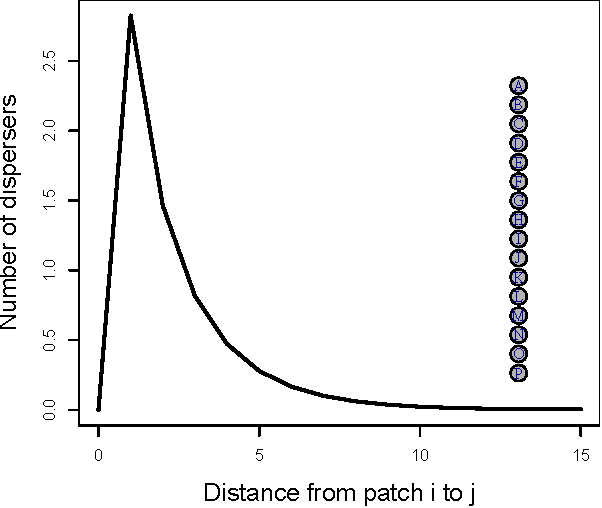
\includegraphics{Managing_for_ecological_surprises_in_metapopulations_files/figure-latex/dispersal-1.pdf}
\caption{Example dispersal patterns across linear network.}
\end{figure}

\subsubsection{Recruitment
stochasticity}\label{recruitment-stochasticity}

\subsubsection{Disturbance}\label{disturbance}

\subsection{Emergent outcomes}\label{emergent-outcomes}

\subsubsection{Scale of management \&
monitoring}\label{scale-of-management-monitoring}

\subsection{Example scenarios}\label{example-scenarios}

\subsection{}\label{section}


\end{document}
